\documentclass[a4paper]{article}

%% Language and font encodings
\usepackage[british]{babel}
\usepackage{graphicx}
\usepackage[T1]{fontenc}
\usepackage[utf8]{inputenc}
\usepackage{lmodern}
\usepackage{graphicx}

%% Sets page size and margins
\usepackage[a4paper,top=3cm,bottom=3cm,left=3cm,right=3cm,marginparwidth=1.75cm]{geometry}
%% To use hyperlinks
\usepackage{hyperref}
%% To use colors
\usepackage[usenames,dvipsnames,svgnames,table]{xcolor}

%% To use maths
\usepackage{amssymb}
\usepackage{amsmath}
\usepackage{mathtools}
\usepackage[linesnumbered,ruled,vlined]{algorithm2e}
\usepackage{titlesec}

%% Command to type a chi character
\DeclareRobustCommand{\rchi}{{\mathpalette\irchi\relax}}
\newcommand{\irchi}[2]{\raisebox{\depth}{$#1\chi$}}
%% Command to simulate a tab character
\newcommand\tab[1][1cm]{\hspace*{#1}}

%% Set sub of subsections
\setcounter{secnumdepth}{4}
\titleformat{\paragraph}
{\normalfont\normalsize\bfseries}{\theparagraph}{1em}{}
\titlespacing*{\paragraph}
{0pt}{3.25ex plus 1ex minus .2ex}{1.5ex plus .2ex}



\title{\textbf{Aprendizagem Autom\'{a}tica} \\
	\large Assignment 2 - Clustering}

\author{Andrea Mascaretti N52222\and Daniel Pimenta N45404}

\begin{document}
	\maketitle
	\begin{abstract}
	The purpose of this assignment was studying and learning the implementation of three major clustering algorithms: K-Means, DBSCAN and Gaussian Mixture Models and
	examine their individual performance in the problem of clustering seismic events.\\
	To achieve this, we varied the main parameter of each algorithm (number of clusters for K-Means, neighbourhood distance $\epsilon$ for DBSCAN and number of gaussian components
	for Gaussian Mixture) and used an internal index (Silhouette score), and external indexes (Rand index, Precision, Recall, F1 measure, Adjusted Rand index, all computed from the fault line information)
	to examine the performance of all three clustering algorithms.\\
	The data set used in this assigment was obtained from the USGS catalog and had the information about all seismic events of magnitude at least 6.5 in the last 100 years.
	In the end, we discussion of the advantages and disadvantages of each algorithm for this dataset, informed by an analysis of their behaviour with different parameters
	and the different scores previously referred.
	TODO brief summary of interpetations and conclusions
	\end{abstract}

	\section{Introduction}
	\subsection{A brief overview of clustering}
	Clustering is the process of examining a collection of "points", and grouping the points into "clusters" according to some distance measure. The goal is for points in the same clusters to have a small distance from one another, while points in different clusters are at a large distance from one another (\cite{9781107077232}).
	In this sense, clustering is helpful when it comes to understanding the structure of the data at hands, especially when dealing with high dimensional datasets. Clustering can provide us with a representation of the data that can facilitate gaining some meaningful insight into their structure. Moreover, it can be applied to reduce complexity and summarise data when this may be needed.\\

	A dataset suitable for clustering is a collection of points $\left\{ \boldsymbol{x}_{i} \right\}_{i=1}^{N} \subset \mathcal{X}$. In a general setting, $\mathcal{X}$ can be any abstract space, but it is often the case that it is a Euclidean space. To perform clustering we need to endow $\mathcal{X}$ with a distance measure (or metric) $\delta$. Note that a metric on a set $\mathcal{X}$ is a function $\delta : \mathcal{X} \times \mathcal{X} \to \left[0,+\infty\right)$ such that for all $x, y, z \in \mathcal{X}$
	\begin{enumerate}
	\item $\delta \left( \boldsymbol{x}, \boldsymbol{y} \right)\geq 0$ (non-negativity)
	\item $\delta \left( \boldsymbol{x}, \boldsymbol{y} \right) = 0 \iff x = y$ (identity of indiscernibles)
	\item $\delta \left( \boldsymbol{x}, \boldsymbol{y} \right) = \delta \left( \boldsymbol{y}, \boldsymbol{x} \right) $ (symmetry)
	\item $ \delta \left( \boldsymbol{x}, \boldsymbol{z} \right) \leq \delta \left( \boldsymbol{x}, \boldsymbol{y} \right) + \delta \left( \boldsymbol{y}, \boldsymbol{z} \right) $ (triangular inequality)
	\end{enumerate}
	Clustering algorithms can be differentiated (some may say \textit{clustered}) into two main different categories, according to the strategy implemented.
	\begin{description}
		\item[Hierarchical clustering] In hierarchical clustering, every point is initially assigned to its own cluster. Clusters are then merged according to their "closeness", where we can use one of the many definitions of the term. The process is ended according to some stopping criteria, for example because we have reached a given number of total cluster input as a threshold or because from merging any of the given clusters we obtain a situation in which data points are too "spread out" according to the definition of "closeness" in use.
		\item[Partitional clustering] In partitional clustering, points are considered in some order and assigned iteratively to the clusters to which the fit best. This phase usually follows another one, during which initial cluster are estimated. Different algorithms in this category allow combining or splitting clusters, or leaving points unassigned when they are \textit{outliers} (i.e., points too far from any cluster).
	\end{description}

	Other two possible classification frameworks, that we mention only briefly, consider other properties:
	\begin{enumerate}
		\item[(a)] We have algorithms that assume that $\mathcal{X}$ is a Euclidean space and others that only consider $\left( \mathcal{X}, \delta \right)$ to be an abstract measure space. In the first case, it is possible to summarise a collection of points by means of a \textit{centroid} - a notion we will introduce later - whereas in the second there is no such thing and we are forced to find a different way to summarise the information contained within a cluster.
		\item[(b)] In this case, the main assumption regards the memory of the machine we are working on. We have two possibilities: we can either assume that the data set is small enough to fit into the main memory or that our data resides in some secondary memory. Sometimes it is infeasible to look at all the pairs of data and strategies must be developed to respond to that. Another problem arising is that of summarising the information contained in every cluster into the main memory for computations.
	\end{enumerate}

	The clustering algorithms considered in this work, namely the K-Means, the DBSCAN and the Gaussian mixture models, are partitional clustering algorithms working in Euclidean spaces. What is more, given the dimensionality of our dataset we will be working on the main memory of the computer, thus avoiding all the issues caused by highly-dimensional data.
	\subsection{Clustering Validation}
	Given the wide variety of existing clustering methods, it is of vital importance to develop objective approaches to validate and assess clustering results. In this sense, three different tasks arise naturally: \textit{clustering evaluation} seeks to estimate the quality of the clustering, \textit{clustering stability} seeks to assess how sensitive a given algorithm is with respect to its parameters and \textit{clustering tendency} aims at understanding whether it is the case to apply clustering in the first place (\cite{zaki2014dataminingbook}).
	We can divide the numerous validity measures and statistics into three main categories.
	\begin{description}
		\item[External] External validation measures employ criteria that are not inherently present in the dataset. For instance, we can have prior or expert-specified clusters.
		\item[Internal] Internal validation measures employ criteria that are based on the data provided for the clustering, such as measure of intra-cluster and inter-cluster dispersion.
		\item[Relative] Relative validation measures aim to directly compare different types of clusterings, usually obtained setting the parameters of one given algorithms in different ways.
	\end{description}
	We hereby introduce five external indices, precision, recall, F1-score, the Rand index and the adjusted Rand index, and one internal index, the silhouette coefficient.
	Before, however, we will require some notations.
	Let $\mathcal{D} = \left\{ \boldsymbol{x}_{j} \right\}_{j=1}^{n} \subset \mathcal{X}$ be a dataset containing $n$ points such that the dimension of $\mathcal{X}$ is equal to $d$, which we have partitioned into $k$ clusters. Let $y_{i} \in \left\{ 1, 2, ..., k \right\} $ denote the ground-truth cluster membership (or label information) for each point. The ground-truth clustering can be expressed as $\mathcal{T} = \left\{ T_{1}, T_{2}, ..., T_{k} \right\}$, where $T_{j} = \left\{ \boldsymbol{x}_{i} \in \mathcal{D} | y_{i} = j \right\}$. Moreover, let $\mathcal{C} = \left\{ C_{1}, ...., C_{r} \right\} $ denote a clustering on the same dataset into $r$ clusters, obtained by means of a certain clustering algorithm. We let $\hat{y}_{i} \in \left\{ 1, 2, ...., r \right\}$ denote the cluster label for $\boldsymbol{x}_{i}$. For the sake of clarity, we shall refer henceforth to $\mathcal{T}$ as \textit{partitioning} and to each $T_{i}$ as \textit{partition}. In a similar fashion, $\mathcal{C}$ will be denoted as a clustering and each $C_{i}$ as a cluster.
	External validation measures try to capture the extent to which points belonging to the same partition appear in the same clusters and, of course, the extent to which points belonging to different partitions are grouped into different clusters. Note that there is usually a trade-off between these two goals, either captured by a measure or implicitly present in its computation.
	External partition relies on the $r \times k$ \textit{contingency table} $N$ that is induced by the clustering $\mathcal{C}$ and the ground-truth partitioning $\mathcal{T}$ defined as follows:
	\begin{equation*}
	N = \left\{ n_{ij} \right\}
	\end{equation*}
	where
	\begin{equation*}
	n_{ij} = | C_{i} \cap T_{j} |.
	\end{equation*}
	In other words, the count $n_{ij}$ denotes the number of points that are common to cluster $C_{i}$ and to the ground-truth partition $T_{j}$.
	Further, we let $n_{i} = \left| C_{i} \right|$ and $m_{j} = \left| T_{j} \right|$.
	Let then $\boldsymbol{x}_{i}, \boldsymbol{x}_{j} \in \mathcal{D}$ be any two points such that $i \neq j$. If both $\boldsymbol{x}_{i}$ and $\boldsymbol{x}_{j}$ belong to the same cluster, or, equivalently, if $\hat{y}_{i} = \hat{y}_{j}$, we call it a \textit{positive} event and if they do not belong to the same cluster, that is if $\hat{y}_{i} \neq \hat{y}_{j}$, we call that a \textit{negative} event. Depending on whether there is agreement between the cluster labels and the partition labels, we thus have four possibilities to consider.
	\begin{itemize}
		\item[True Positives] $\boldsymbol{x}_{i}$ and $\boldsymbol{x}_{j}$ belong both to the same partition in $\mathcal{T}$ and to the same cluster in $\mathcal{C}$. We have a true positive pair because the positive event correspond to the ground truth.
		\begin{equation*}
		TP = \left|\left\{\left(\boldsymbol{x}_{i}, \boldsymbol{x}_{j}\right) : y_{i} = y_{j}, \hat{y}_{i} = \hat{y}_{j} \right\}\right|
		\end{equation*}
		\item[False Negatives] $\boldsymbol{x}_{i}$ and $\boldsymbol{x}_{j}$ belong to the same partition in $\mathcal{T}$ but to different clusters in $\mathcal{C}$. Thus, the negative event does not correspond to the truth.
		\begin{equation*}
		FN = \left|\left\{\left(\boldsymbol{x}_{i}, \boldsymbol{x}_{j}\right) : y_{i} = y_{j}, \hat{y}_{i} \neq \hat{y}_{j} \right\}\right|
		\end{equation*}
		\item[False Positives] $\boldsymbol{x}_{i}$ and $\boldsymbol{x}_{j}$ do not belong to the same partition in $\mathcal{T}$ but they do belong to the same cluster in $\mathcal{C}$. The positive event is therefore false.
		\begin{equation*}
		FP = \left|\left\{\left(\boldsymbol{x}_{i}, \boldsymbol{x}_{j}\right) : y_{i} \neq y_{j}, \hat{y}_{i} = \hat{y}_{j} \right\}\right|
		\end{equation*}
		\item[True Negative] $\boldsymbol{x}_{i}$ and $\boldsymbol{x}_{j}$ neither belong to the same partition in $\mathcal{T}$ nor to the same cluster in $\mathcal{C}$. The false event is therefore true.
		\begin{equation*}
		TN = \left|\left\{\left(\boldsymbol{x}_{i}, \boldsymbol{x}_{j}\right) : y_{i} \neq y_{j}, \hat{y}_{i} \neq \hat{y}_{j} \right\}\right|
		\end{equation*}
		\end{itemize}
		The total pair of points is given by $N = \frac{n\left(n-1\right)}{2}$ and we have the following identity:
		\begin{equation*}
		N = TP + FN + FP + TN.
		\end{equation*}
		A naive computation of the preceding four cases requires $O\left(n^{2}\right)$ time. However, there is a more efficient way to proceed with the calculations, considering the contingency table $N = \left\{ n_{ij} \right\}$ with $1 \leq i \leq r$ and $1 \leq j \leq k$. The number of true positives is then
		\begin{equation*}
		TP = \sum_{i=1}^{r} \sum_{j=1}^{k} {{n_{ij}}\choose{2}} = \sum_{i=1}^{r} \sum_{j=1}^{k} \frac{n_{ij}\left(n_{ij} - 1\right)}{2}  = \frac{1}{2} \left( \sum_{i=1}^{r} \sum_{j=1}^{k} n_{ij}^{2} - \sum_{i=1}^{r} \sum_{j=1}^{k} n_{ij} \right) = \frac{1}{2} \left( \left( \sum_{i=1}^{r} \sum_{j=1}^{k} n_{ij}^{2} \right) - n \right).
		\end{equation*}
		This follows from the fact that each pair of points among the $n_{ij}$ share the same cluster label $i$ and the same partition label $j$ and of course the last step follows from the fact that $\sum_{i=1}^{r} \sum_{j=1}^{k} = n$.
		To compute the total number of false negatives, we have to remove the number of true positives from the number of pairs that belong to the same partition. Because two points $\boldsymbol{x}_{i}$ and $\boldsymbol{x}_{j}$ that belong to the same partition have $y_{i} = y_{j}$, if we remove true positives we are left with pairs for which $\hat{y}_{i} \neq \hat{y}_{j}$, which is exactly the false negatives.
		This yields
		\begin{equation*}
		FN = \sum_{j=1}^{k} {{m_{ij}}\choose{2}} - TP = \frac{1}{2} \left( \sum_{j=1}^{k} m_{j}^{2} - \sum_{j=1}^{k} m_{j} - \sum_{i=1}^{r}\sum_{j=1}^{k} n_{ij}^{2} + n \right) = \frac{1}{2} \left( \sum_{j=1}^{k} m_{j}^{2} - \sum_{i=1}^{r} \sum_{j=1}^{k} n_{ij}^{2} \right).
		\end{equation*}
		The number of false positives can be obtained in a very similar fashion:
		\begin{equation*}
		FP = \sum_{i=1}^{r} {n_{i}\choose{2}} - TP = \frac{1}{2}\left( \sum_{i=1}^{r} n_{i}^{2} - \sum_{i=1}^{r} \sum_{j=1}^{k} n_{ij}^{2} \right).
		\end{equation*}
		To conclude, we can find the true negatives by doing
		\begin{equation*}
		TN = N - \left( TP + FN + FP \right) = \frac{1}{2} \left( n^{2} - \sum_{i=1}^{r} n_{i}^{2} - \sum_{j=1}^{k} m_{j}^{2} + \sum_{i=1}^{r} \sum_{j=1}^{k} n_{ij}^{2} \right).
		\end{equation*}
		In this way, we can compute the values in $O\left(rk\right)$ time. As the contingency table can be obtained in linear time, the total time is $O\left(n + rk\right)$.
		Having said that, we can proceed to define the external indices we shall be using throughout our analysis.
		\begin{description}
			\item[Precision] Precision, in the context of information retrieval, is defined as the fraction of retrieved documents that are relevant. We define it by analogy here as
			\begin{equation*}
			\frac{TP}{TP + FP},
			\end{equation*}
			obtaining an index that gives us the fraction of true, or correctly classified, point pairs compared to all the point pairs in the same clusters. Note that the index will always be contained in $\left[0,1\right]$.
			\item[Recall] Recall, in the context of information retrieval, is defined as the fraction of relevant documents that are actually retrieved. As done before, we define it by analogy
			\begin{equation*}
			\frac{TP}{TP + FN}.
			\end{equation*}
			Here we measure the fraction of correctly labelled points pairs compared to all the points pairs in the same partition. Note that the index will always be contained in $\left[0,1\right]$.
			\item[F1-Score] The F1-Score is defined to be the harmonic mean between precision and recall:
			\begin{equation*}
			2\frac{precision \cdot recall}{precision + recall}
			\end{equation*}
			When both recall and precision are perfect, the value is $1$ and is bounded below by $0$.
			\item[Rand Statistics] The Rand statistics measures the fraction of true positive and true negatives over all point pairs. It is defined as
			\begin{equation*}
			Rand = \frac{TP+ TN}{N}.
			\end{equation*}
			The Rand statistics measures the fraction of point pairs where both $\mathcal{C}$ and $\mathcal{T}$ agree. A perfect clustering has a value of 1 for the statistics.
			\item[Adjusted Rand Index] The adjusted Rand index builds on the Rand index, correcting it for chance. It can yield negative values and it is defined as
			\begin{equation*}
			Adjusted Rand Index = \frac{\sum_{i=1}^{r} \sum_{j=1}^{k} {n_{ij}\choose{2}} - \frac{\sum_{i=1}^{r}{n_{i}\choose{2}}  \sum_{j=1}^{k}{m_{j}\choose{2}}}{{{n}\choose{2}}}}{\frac{1}{2}\left[\sum_{i=1}^{r} {{n_{i}}\choose{2}} + \sum_{j=1}^{k} {{m_{j}}\choose{2}} \right] - \frac{\left[\sum_{i=1}^{r} {{n_{i}}\choose{2}}  \sum_{j=1}^{k} {{m_{j}}\choose{2}} \right]}{{{n}\choose{2}}}}
			\end{equation*}
		\end{description}
	We now move on to describing the internal index we are going to use.
	\begin{description}
		\item[Silhouette Coefficient] The silhouette coefficient is a measure of cohesion and separation of clusters. It is based on the difference between the average distance to points in the closest cluster and to points in the same clusters. For each point $\boldsymbol{x}_{i}$, we calculate its silhouette coefficient $s_{i}$ as
		\begin{equation*}
		s_{i} = \frac{\mu_{out}^{\min}\left(\boldsymbol{x}_{i}\right) - \mu_{in}\left(\boldsymbol{x}_{i}\right)}{\max\left\{\mu_{out}^{\min}\left(\boldsymbol{x}_{i}\right), \mu_{in}\left(\boldsymbol{x}_{i}\right) \right\}},
		\end{equation*}
		where $\mu_{in}\left( \boldsymbol{x}_{i} \right)$ is the mean distance from $\boldsymbol{x}_{i}$ to points in its own cluster $\hat{y}_{i}$:
		\begin{equation*}
		\mu_{in}\left( \boldsymbol{x}_{i} \right) = \frac{\sum_{\boldsymbol{x}_{j} \in C_{\hat{y}_{i}}, j \neq i} \delta \left(\boldsymbol{x}_{i}, \boldsymbol{x}_{j}\right)}{n_{\hat{y}_{i}} - 1}
		\end{equation*}
		and
		\begin{equation*}
		\mu_{out}^{\min} \left(\boldsymbol{x}_{i}\right) = \min_{j \neq \hat{y}_{i}} \left\{ \frac{\sum_{\boldsymbol{y} \in C_{j}} \delta \left(\boldsymbol{x}_{i}, \boldsymbol{y}\right)} {n_{j}} \right\}
		\end{equation*}
		The $s_{i}$ value of a point always lies in the interval $\left[-1,1\right]$. A value closer to $+1$ indicates that $\boldsymbol{x}_{i}$ is much closer to points in its own cluster than to points in other clusters. A value close to zero indicates that $\boldsymbol{x}_{i}$ is close to the boundary and a value close to $-1$ indicates that $\boldsymbol{x}_{i}$ is closer to another cluster than it is to its own.
		The silhouette coefficient is defined as
		\begin{equation*}
		SC = \frac{1}{n} \sum_{i=1}^{n} s_{i}
		\end{equation*}
		and, as it is natural, a value close to $+1$ indicates a good clustering.
	\end{description}
	\subsection{The USGS Catalog}
	The dataset on which we shall develop our analysis was obtained from the \href{https://earthquake.usgs.gov/earthquakes/search/}{USGS catalog}. It comprises all the geographical coordinates of every seismic event of a magnitude of at least 6.5 occurred during the past century. A column, specifying the fault line between the tectonic plates that are closest to the seismic event was also considered. It was obtained from the same source and it will serve the role of providing a ground-truth partitioning for external validation. Each fault line is identified by an non-negative integer, with the exception of those earthquakes that were not significantly close to any fault line: they are labelled as $-1$.
	Before proceeding with the analysis, we transformed the longitude and latitude values into Earth-centred, Earth-fixed coordinates $\left(x,y,z\right)$ as follows:
	\begin{equation*}
	x = R \, \cos\left(latitude \cdot \frac{\pi}{180}\right) \cos\left(longitude \cdot \frac{\pi}{180} \right)
	\end{equation*}
	\begin{equation*}
	y = R \, \cos\left(latitude \cdot \frac{\pi}{180}\right) \sin\left(longitude \cdot \frac{\pi}{180} \right)
	\end{equation*}
	\begin{equation*}
	z = R \, \sin\left(latitude \cdot \frac{\pi}{180}\right),
	\end{equation*}
	where $R = 6731 \, \mathrm{Km}$, being the average radius of the Earth. This was done as necessary to compute distances between two points.
	Apart from that, no other transformation was added to the data: we did not scale them, as all the axes are measured according to the same unit (namely kilometres).

	The analysis was conducted using the \href{https://www.python.org/}{Python} programming language. In particular, the \href{http://scikit-learn.org/stable/}{Scikit-Learn} package (\cite{scikit-learn}), the \href{http://www.numpy.org/}{NumPy} package (\cite{doi:10.1109/MCSE.2011.37}) and the \href{https://matplotlib.org/}{Matplotlib} package (\cite{Hunter_2007}) were used.
	\section{Clustering Algorithms}
	\subsection{K-Means Algorithm}
	In our exposition of the K-Means Algorithm we rely heavily on \cite{hastie01statisticallearning}, \cite{MR2372475} and \cite{zaki2014dataminingbook}.
	Suppose that we have a set of $n$ observations, indexed by $I = \{1, ..., n\}$, of some quantitative
	variables
	$$ C = \{ \boldsymbol{x}_{1}, \boldsymbol{x}_{2}, ..., \boldsymbol{x}_{n} \} $$
	where

	$$ \boldsymbol{x}_{i} \in \mathbb{R}^{p},\;\forall i\in I$$


	We also have a set of labels (at this stage we will consider their
	number as given and such that $card(\mathcal{L})=k,\:k\in\left[1,n\right]\cap\mathbb{N}$)

	$$
	\mathcal{L}=\left\{ l_{1},\ldots,l_{k}\right\} ,\;K:=\left\{ 1,\ldots,k\right\}
	$$
	Our goal is to construct a (\textit{measurable}) function to associate each
	and every element of $C$ to one label in $\mathcal{L}$. It is easy
	to see that it makes no difference to work with $\mathcal{L}$ or
	$K$ as we can always find a bijection between the two sets.

	We have reasons to believe that the elements belonging to one particular
	group are somewhat more similar to each other than they are to members
	of other groups and that one element can belong to one group and one
	group only. We also hypothesise that there are no empty groups. Translating
	this into mathematical terms, our aim is to find a collection

	$$ 	\left\{ C_{i}\right\} _{i\in K}	$$

	such that
	$$ C_{i}\cap C_{j}=\emptyset,\;i\neq j $$

	and

	$$
	\bigcup_{i=1}^{k} C_{i} = C
	$$
	or, in other words, we want to partition $C$ into $k$ clusters.

	Moreover, for each cluster we wish to find a representative member to summarise the information contained within the cluster. An usual choice is to consider the mean, or \textbf{centroid}, of the cluster defined as
	\begin{equation*}
	\boldsymbol{c}_{i} = \frac{1}{n_{i}} \sum_{\boldsymbol{x}_{j} \in C_{i}} \boldsymbol{x}_{j},
	\end{equation*}
	where $n_{i}$ is the cardinality of $C_{i}$.\\

	The main issue is to find a method to partition the set $C$ into
	the clusters. A brute-force algorithm for finding a good clustering would imply generating all the possible partition of $n$ points into $k$ cluster and then, once an evaluation function has been set, take the best one. Informally, however, we can see that each point can be assigned to any of the $k$ clusters so that there are at most $k^{n}$ possible clusterings. Considering that any permutation of the $k$ clusters within a given clustering yields an equivalent result, we see that there are $O(\frac{k^{n}}{k!})$ clusterings of $n$ points into $k$ clusters. It is therefore clear that we need to rely on a different strategy.\\


	First of all, we need to define in a more precise manner
	the meaning of similarity between two points: we will consider the squared \textsl{Euclidean
		distance} for this purpose
	$$
	d(\boldsymbol{x}_{i},\boldsymbol{x}_{j})= \sum_{k = 1}^{p} \left( x_{ik} - x_{jk}
	\right)^{2}.
	$$
	We now need to define some \textsl{loss} function and try to minimise
	it. The most natural idea follows from the assumption that members
	of one given cluster will be closer to each other than to member of
	other clusters: this is equivalent to stating that the correct partitioning
	will minimise the variability \textsl{within} the clusters. We need
	to translate this key concept into an objective function.

	We define
	$$
	I_{k}:=\left\{ i\in I\:s.t.\:\boldsymbol{x}_{i}\in C_{k}\right\}
	$$

	and in this case we will have
	$$
	W(C_{k}) = \frac{1}{n_{k}} \underset{i,j\in I_{k}}{\sum} \sum_{l=1}^{p} \left(x_{il}-x_{jl}\right)^{2}
	$$
	and the problem becomes as follows
	\footnote{It is important to notice that this function surely decreases for
		increasing $k$ and in the extreme case of $k=n$ we have that each
		cluster contains only one point and we have no variability whatsoever.
		It is important to understand that we are looking for classes that
		do have some internal variability.}
	$$	\underset{C_{1},\ldots,C_{k}}{\min}\left\{ \sum_{k=1}^{K}W(C_{k})\right\} $$


	To solve the problem, K-Means applies a greedy iterative algorithm to find a local optimum.

	The centroids are randomly generated into the data space, usually considering a uniform distribution between the range for each dimension. Every iteration, then, consists of two main steps: $(1)$ cluster assignment and $(2)$ centroid update. That is to say, given the $k$ cluster means, in the cluster assignment step, each point $\boldsymbol{x}_{j}$ is assigned to the closest mean, which induces a clustering (each cluster $C_{i}$ comprises all the points that are closer to $\boldsymbol{c}_{i}$ than to any other centroid).
	\begin{equation*}
	i^{*}=\arg\underset{i\in K}{ \min}\left\{ d(\boldsymbol{x}_{j},\boldsymbol{c}_{i})\right\} =\arg\min_{i \in K}\left\{ d(\boldsymbol{x}_{j},\boldsymbol{c}_{1}),\ldots,d(\boldsymbol{x}_{j},\boldsymbol{c}_{k})\right\} \:\Longrightarrow\:\boldsymbol{x}_{j}\in C_{i^{*}}
	\end{equation*}
	Now, given a set of cluster $C_{i},\, i=1,...,k$, in the centroid update step new values are computed for each cluster from the points in $C_{i}$. The cluster assignment and centroid update steps are repeated until we reach a fixed point or a local minimum. In more practical words, we can say that K-Means converges if the centroids do not change from one iteration to the next and we can stop when the distance between an iteration and another is smaller than some positive threshold $\varepsilon$.

	The algorithm we have just defined is descent, that is it improves
	the solution at each iteration so that when the termination condition
	is true, we are certain to have reached a \textsl{local optimum}.
	Considering also that we randomly set the initial centroids, it is a good practice to run the algorithm several time and report the clustering with the evaluation value. It is also worth noting that K-Means generates convex-shaped clusters as the region in the data space corresponding to each cluster can be obtained intersecting the half-spaces resulting from the hyperplanes that bisect and are normal to the segments that join pairs of centroids.

	There is also one last important point to state. Any time we perform
	the K-means methods, we will find $k$ clusters on our data. Now,
	the question is: are we really separating actual subgroups or are
	we just \textsl{clustering the noise}? Moreover, suppose that we are
	dealing with a case in which the vast majority of data belongs to
	a small number of subgroups, but for a small subset that is quite
	different from the rest. As our method \textsl{forces} our data into
	a fixed number of clusters, the presence of an outlying class might
	bring to distorted results. So it is good practice not only to try
	various values of $k$ to see what happens, but also to try and apply
	to algorithm to subsets of our initial set to check that results remain
	somewhat stable.

	\subsubsection{Algorithm for K-means Clustering}
	\begin{enumerate}
		\item Randomly assign a number, from 1 to K, to each observation: they will
		serve as initial cluster assignments. Set $\mu:=0$
		\item Iterate what follows until termination criterion holds:
		\begin{enumerate}
			\item For each cluster, compute the \textsl{centroid}
			$$
			\boldsymbol{c}_{i}^{\mu}=\frac{1}{card(C_{i}^{\mu})}\underset{j\in I_{i}^{\mu}}{\sum}\boldsymbol{x}_{i},
			$$
			computed as the mean vector of the observations in the $k$-th cluster
			at $\mu$-th iteration
			\item Assign each observation to the cluster whose centroid is closest (with
			respect to the Euclidean distance) as follows
			$$
			\forall j\in I,\;i^{*}=\underset{i\in K}{\min}\left\{ d(\underline{x}_{j},\underline{c}_{i}^{\mu})\right\} =\min\left\{ d(\underline{x}_{j},\underline{c}_{1}^{\mu}),\ldots,d(\underline{x}_{j},\underline{c}_{k}^{\mu})\right\} \:\Longrightarrow\:\underline{x}_{j}\in C_{i^{*}}^{\mu}
			$$
			\item Set $\mu:=\mu+1$
		\end{enumerate}
		\item Termination occurs when cluster assignments stop changing
	\end{enumerate}

	\subsubsection{Choosing the number of clusters}
	In order to choice the number of clusters that seemed to yield the best results, we decided to run the algorithm for different values of $k$, from $1$ to $100$. The results are shown in Figure \ref{fig:kmeans}.
	First of all, we can point out that there appear to be an inverse correlation between precision and recall, as expected. In facts, as the number of clusters grows we have an increased rate of false negatives. This is given to the fact that the increased number of clusters makes it more likely to have points belonging to the same partition that are classified into different clusters. On the other hand, increasing $k$ implies a decrease in false positives as it is more unlikely that points belonging to the same partition are clustered into different clusters.
	The trade-off is also evident considering the F1-Score, that performs better when we have high recall and a good value for the precision (that could anyway improve allowing for greater $k$).
	It is interesting to see that the number of clusters suggested by precision and recall are very different. In this sense, the best choice depends very much on what it is important to maximise: whether it is the fraction of positive events that are true compared to the point in the same cluster or the fraction of correctly labelled point within a cluster with respect to al the points pairs in the same partition.
	The Rand index and the adjuster Rand index suggests a similar number of clusters (if we consider the number that we obtain considering the "elbow" in the Rand index plot). However, we see how the adjusted Rand index deteriorates when we pass that number: it is due to the correction for chance done by the index.
	As far as the Silhouette coefficient is concerned, we see that we obtain again a suggested value between $20$ and $40$, where we have a good balance between cohesion and separation of clusters. We obtain a result that substantially agree with the last three external indices.
	This may be due to the intrinsic nature of the K-Means algorithm, that has to rely on convex-shaped clusters and cannot therefore adapt too much to the domain at hands, characterised by rather "prolonged" clusters in shape (as it is often the case with geophysical data): with a small number of clusters we have a good recall, that we pay in terms of precision, and as soon as we try to augment it we see that we lose in terms of fidelity to the original partitioning.
	We provide a representation of the clustering induced (Figure \ref{fig:kmeans_world}) considering the best value obtained by means of the Silhouette score, which should not be too different from the clustering induced by the F1-Score, the Rand index and the adjusted Rand index as already explained.
	In Table \ref{table:kmeans}, we report the indices we obtain maximising for each of them.\\

	\begin{table}[h!]
		\centering
		\begin{tabular}{l*{6}{c}r}
			Index              & Precision & Recall & F1-Score & Rand Index & Adjusted Rand Index  & Silhouette Score & $k$ \\
			\hline
			Prec. 		& 0.761 & 0.093 & 0.166 & 0.502 & 0.147 & 0.496 & 146  \\
			Recall          & 0.127 & 0.791 & 0.219 & 0.326 &  0.056 & 0.481 &  2  \\
			F1-Sc.        & 0.347 & 0.667 & 0.457 & 0.483 &  0.374 & 0.374 &  6  \\
			Rand Ind.      & 0.619 & 0.244 & 0.350 & 0.503 &  0.311 & 0.516 &  39  \\
			Adj. Rand Ind. & 0.575 & 0.352 & 0.437 & 0.503 &  0.390 & 0.507 &  22  \\
			Silh. Score & 0.524 & 0.299 & 0.380 & 0.501 &  0.332 & 0.528 &  25  \\
		\end{tabular}
	\caption{Values of the Precision, Recall, F1-Score, Rand index, adjusted Rand index and Silhouette score at the $k$ maximising the index considered in the row.}
	\label{table:kmeans}
	\end{table}


	\begin{figure}
		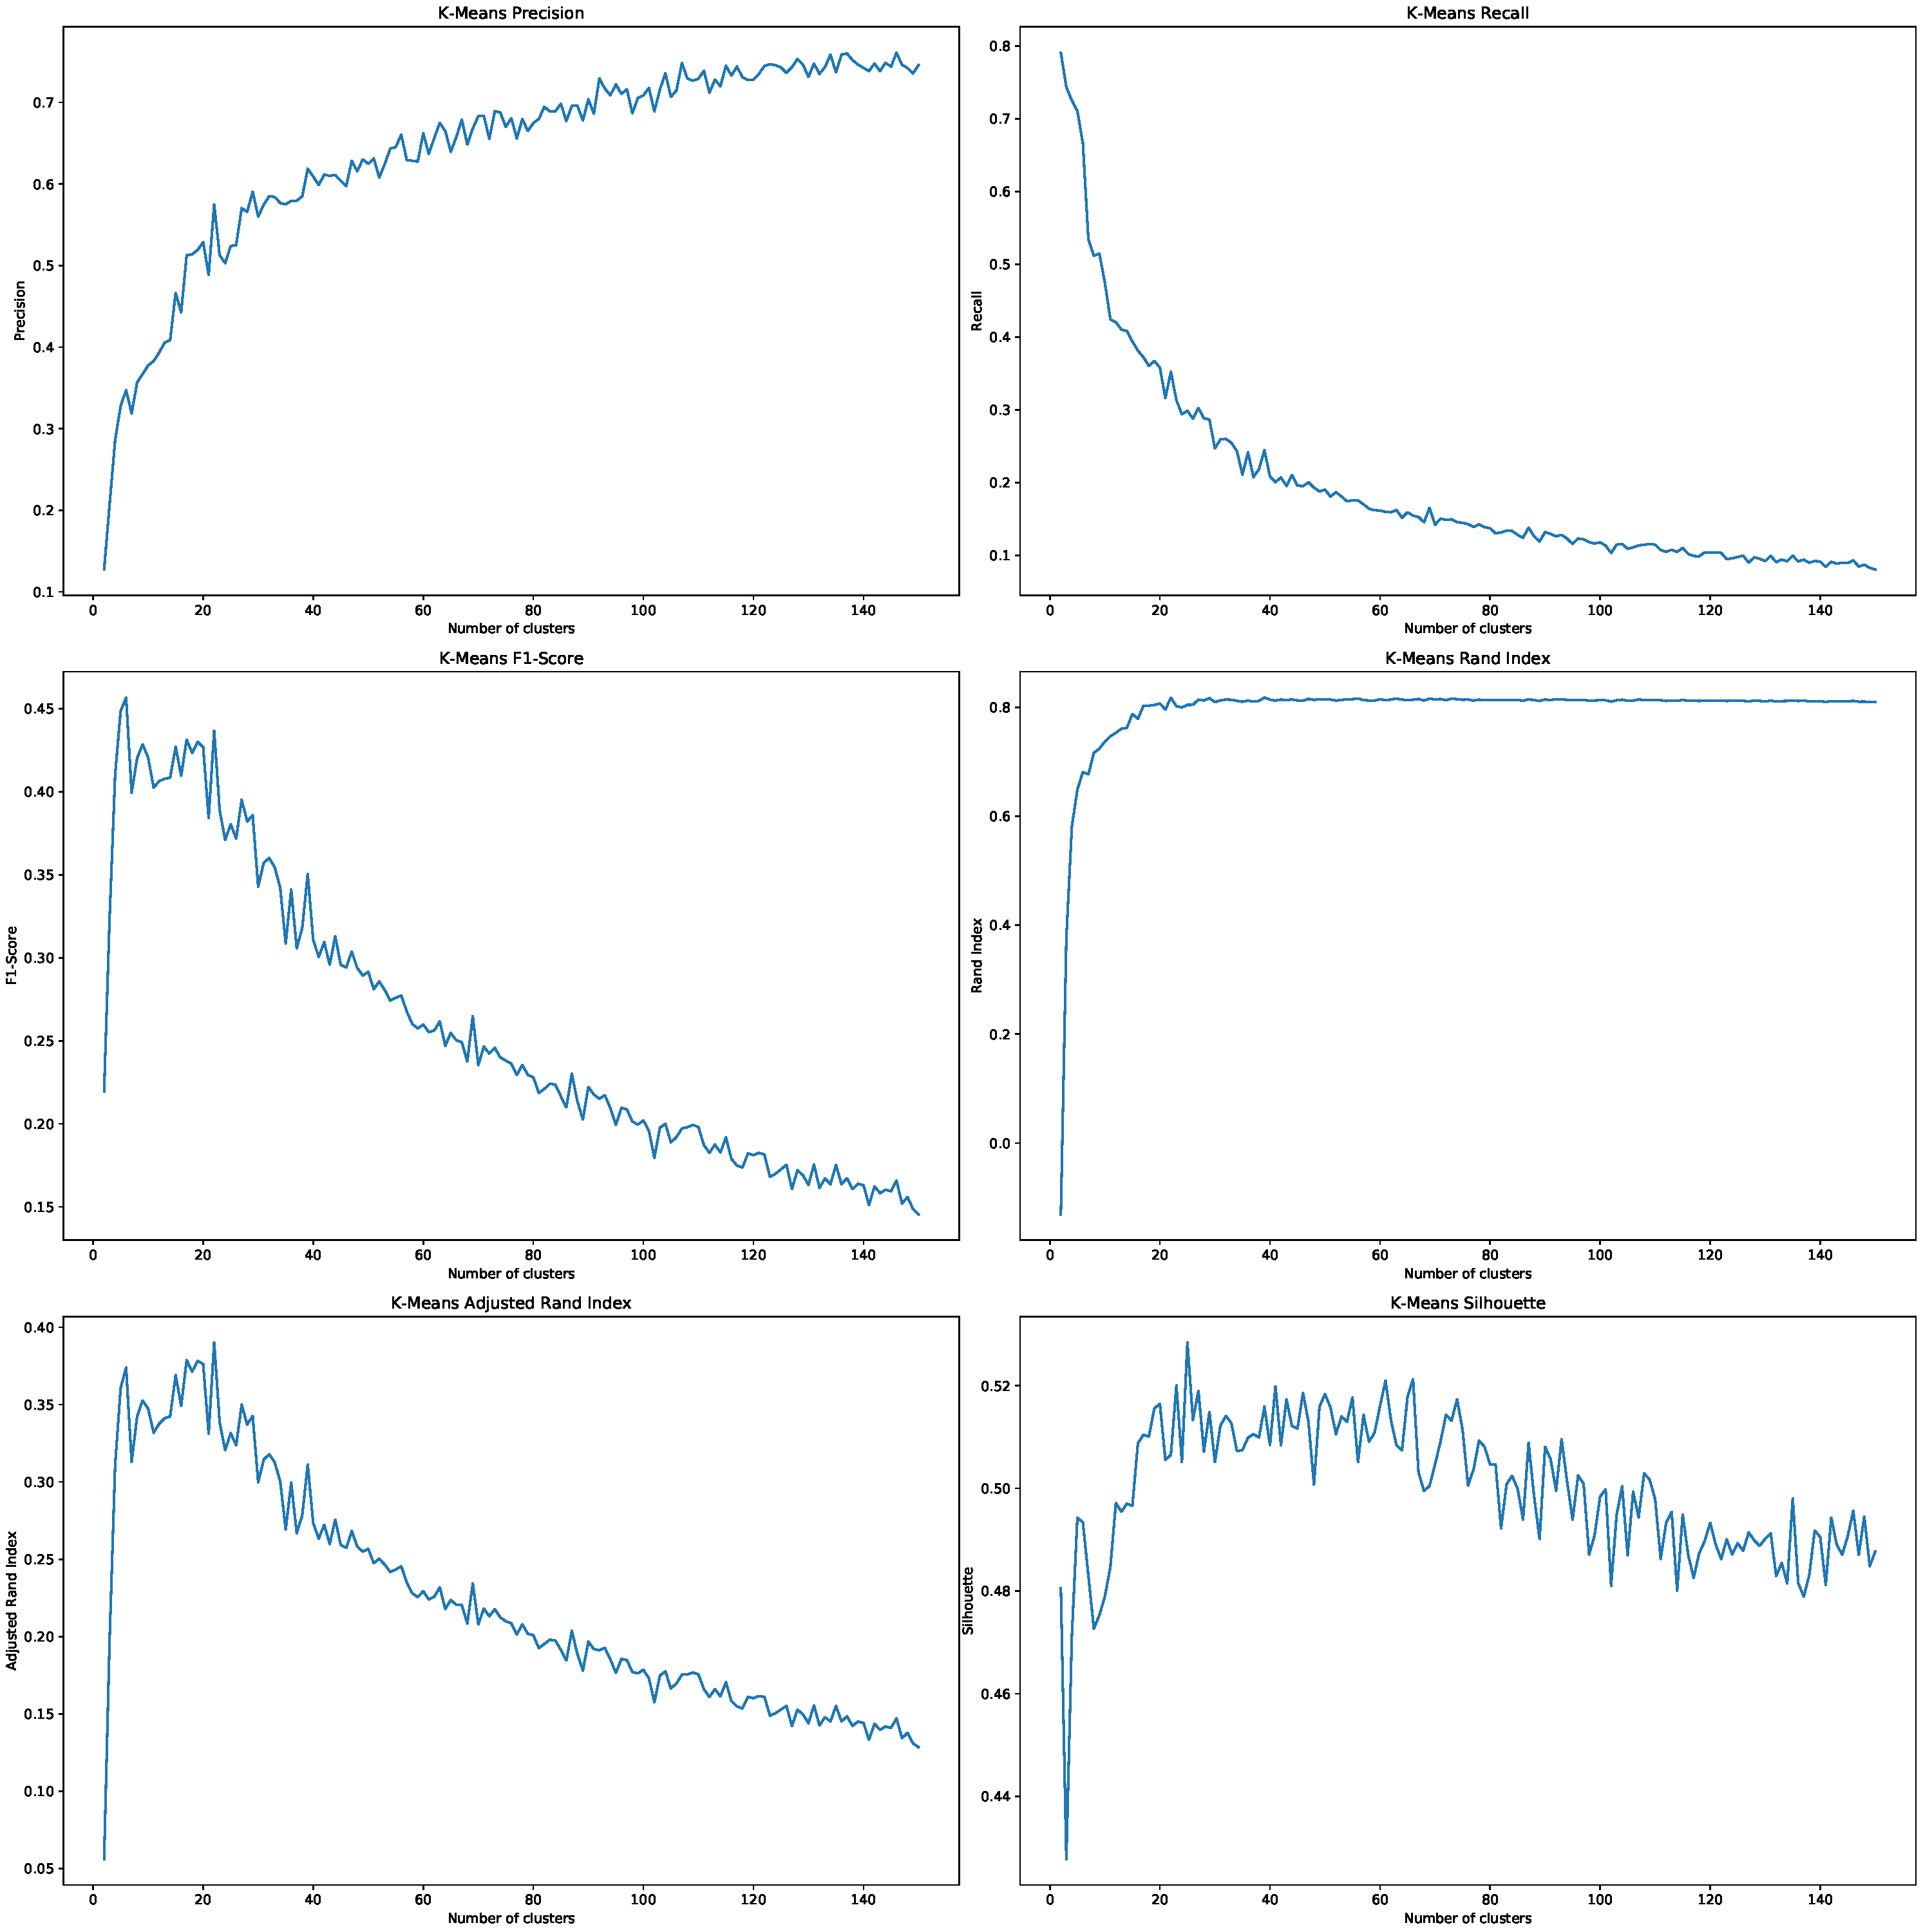
\includegraphics[width=\linewidth]{kmeans_indeces.pdf}
		\caption{Precision, Recall, F1-Score, Rand Index, Adjusted Rand Index and Silhouette Score for the K-Means algorithms at different values of $k$.}
		\label{fig:kmeans}
	\end{figure}
	\begin{figure}
		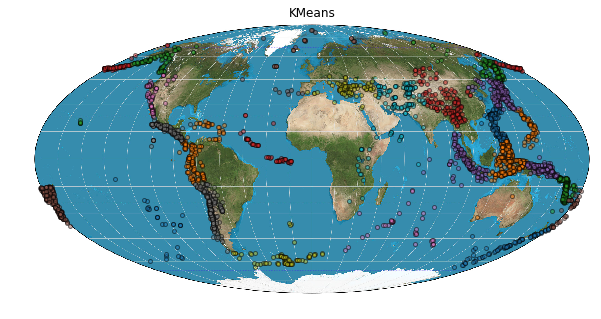
\includegraphics[width=\linewidth]{kmeans_world.png}
		\caption{Representation of the clustering obtained applying the K-Means algorithm with $k= 25$.}
		\label{fig:kmeans_world}
	\end{figure}

	\subsection{DBSCAN}
	In our analysis of the DBSCAN algorithm, we shall be relying mainly on \cite{Ester96adensity-based} and \cite{zaki2014dataminingbook}. The necessity of an algorithm adopting a different philosophy with respect to that of the K-Means algorithm arises from the fact that representative methods (such as the latter or, for instance, EM methods) are suitable for finding, at best, convex clusters.
	However, for non-convex clusters these methods are not capable to find the true clusters. This is because two points belonging to two different clusters might actually be close to each others than two points from the same on.
	For this reason, density-based clustering algorithms adopt a different paradigm, using the local densities of points to determine the clusters rather than relying solely on distances between couple of them.

	We now introduce some preliminary concepts. First of all, we define a \textbf{ball} of radius $\varepsilon$ around a point $\boldsymbol{x} \in \mathbb{R}$, called \textit{$\varepsilon$-neighbourhood} of $\boldsymbol{x}$, as follows:
	\begin{equation*}
	\mathcal{N}_{\varepsilon} (\boldsymbol{x}) = B_{\delta}\left( \boldsymbol{x}, \varepsilon \right) = \left\{ \boldsymbol{y} \; s.t. \; \delta \left( \boldsymbol{x}, \boldsymbol{y} \right) \leq \varepsilon \right\}.
	\end{equation*}
	Here $\delta \left( \boldsymbol{x}, \boldsymbol{y} \right)$ represents the distance between the points $\boldsymbol{x}$ and $\boldsymbol{y}$, which is usually assumed to be the Euclidean distance, that is
	\begin{equation*}
	\delta(\boldsymbol{x}, \boldsymbol{y}) = || \boldsymbol{x} - \boldsymbol{y} ||_{2}.
	\end{equation*}
	However, other distance metrics can be used.
	For any point $\boldsymbol{x} \in \boldsymbol{D}$, where $\boldsymbol{D}$ is the set of data points, we say that $\boldsymbol{x}$ is a \textit{core point} if there are at least $k$ points in its $\varepsilon$-neighbourhood.
	In other words, $\boldsymbol{x}$ is defined as a core point when it holds:
	\begin{equation*}
	| \mathcal{N}_{\varepsilon}(\boldsymbol{x})| \geq k,
	\end{equation*}
	where $k$ is a local density (or frequency) threshold defined by the user.

	A \textit{border point} is defined as a point that does not meet the $k$ threshold or, equivalently, that is such that $|\mathcal{N}_{\varepsilon}(\boldsymbol{x})| < k$, but belongs to the $\varepsilon$-neighbourhood of some core point $\boldsymbol{z}$.
	Finally, if a point is neither a core point nor a border point, it is called a \textit{noise point} or outlier.
	We say that a point $\boldsymbol{x}$ is \textit{directly density reachable} from another point $\boldsymbol{y}$ if $\boldsymbol{x} \in \mathcal{N}_{\varepsilon} \left( \boldsymbol{y} \right)$ and $\boldsymbol{y}$ is a core point.
	We say that $\boldsymbol{x}$ is \textit{density reachable} from $\boldsymbol{y}$ if there exists a chain of point, $\boldsymbol{x}_{0}, \boldsymbol{x}_{1}, ..., \boldsymbol{x}_{l}$, such that $\boldsymbol{x}=\boldsymbol{x}_{0}$ and $\boldsymbol{y} = \boldsymbol{x}_{l}$, and $\boldsymbol{x}_{i}$ is directly density reachable from $\boldsymbol{x}_{i-1}$ for all $i=1,...,l$.
	In other words, there must be a set of core points leading from $\boldsymbol{y}$ to $\boldsymbol{x}$. Note that the relationship of density reachability is an asymmetric property (or a directed relationship).
	Define any two points $\boldsymbol{x}$ and $\boldsymbol{y}$ to be density connected if there exists a core point $\boldsymbol{z}$, such that both $\boldsymbol{x}$ and $\boldsymbol{y}$ are density reachable from $\boldsymbol{z}$.
	A \textit{density based cluster} is defined as a maximal set of density connected points.

	The algorithm works as follows. First, DBSCAN computes the $\varepsilon$-neighbourhood $\mathcal{N}_{\varepsilon} \left( \boldsymbol{x}_{i} \right)$ for each point $\boldsymbol{x}_{i} \in \boldsymbol{D}$. It then checks if $\boldsymbol{x}_{i}$ is a core point. Moreover, it sets the cluster id $id\left(\boldsymbol{x}_{i}\right) = \emptyset$ for all points, indicating that they are not assigned to any cluster.
	Next, starting from each core point that is not assigned, the algorithm recursively finds all its density connected points, which are assigned to the same clusters. Some border point may be reachable from core points in more than on cluster: they may either be arbitrarily assigned to one of the clusters or to all of them (if overlapping clusters are allowed!).
	Those points that do not belong to any cluster are treated as outliers or noise.
	DBSCAN can be viewed from another point of view. In fact, we can see it as a search for connected components in a graph with the following characteristics: the vertices corresponds to the core points in the dataset and there exists an (undirected) edge between two vertices (core points) if the distance between them is less than $\varepsilon$, that is to say, if each of them is in the $\varepsilon$-neighbourhood of the other point.
	The connected components of this graph correspond to the core points of each cluster. Next, every core point incorporates into its cluster any border points in its neighbourhood.
	The biggest drawback of DBSCAN is given by its sensitivity to the value of $\varepsilon$, in particular if clusters have different densities. What happens is that is $\varepsilon$ is too small, than sparser clusters will be categorised as noise and if it is too large different clusters might end up being grouped together.

	\subsection{Gaussian Mixture}
	In order to introduce Gaussian Mixture models, we shall be relying mainly on \cite{Bishop:2006}.
	A Gaussian mixture distribution can be written as a linear superposition of Gaussians in the form
	\begin{equation}\label{eqn::gauss_mix}
	p(\boldsymbol{x}) = \sum_{k=1}^{K} \pi_{k} \mathcal{N} \left( \boldsymbol{x}  | \boldsymbol{\mu}_{k}, \Sigma_{k} \right)
 	\end{equation}

 	However, it is possible to rewrite \eqref{eqn::gauss_mix} as follows. Let us a introduce a $K$-dimensional binary random variable $\boldsymbol{z}$ having a $1$-of-$K$ representation so that a particular element $z_{k}=1$ and all the other elements are equal to $0$. We have that $\sum_{k} z_{k} = 1$ and that, for all $k$, $z_{k} \in \{ 0, 1 \}$. We can see that there are $K$ possible states for which no element of $\boldsymbol{z}$ is zero.
 	We now proceed to defining the joint distribution of $p(\boldsymbol{x}, \boldsymbol{z})$ as $p(\boldsymbol{x}|\boldsymbol{z})p(\boldsymbol{z})$.
 	We set
 	\begin{equation*}
 	p(z_{k} = 1) = \pi_{k},
 	\end{equation*}
 	with $ \pi_{k} \in \left[0,1 \right] $ and $\sum_{k=1}^{K} \pi_{k} = 1 $, which we can rewrite
 	\begin{equation*}
 	p(\boldsymbol{z}) = \prod_{k=1}^{K} \pi_{k}^{z_{k}}.
 	\end{equation*}
 	Similarly, we the conditional distribution of $\boldsymbol{x}$ given $\boldsymbol{z}$ is
 	\begin{equation*}
 	p(\boldsymbol{x}|z_{k} = 1) = \mathcal{N} \left( \boldsymbol{x} | \boldsymbol{\mu}, \Sigma_{k} \right).
 	\end{equation*}
 	We can rewrite the last equation as
 	\begin{equation*}
 	p(\boldsymbol{x}|\boldsymbol{z}) = \prod_{k=1}^{K} \mathcal{N} (\boldsymbol{x} | \boldsymbol{\mu}, \Sigma_{k})^{z_{k}}.
 	\end{equation*}
 	The conditional distribution of $\boldsymbol{z}$ given $\boldsymbol{x}$ is computed considering the theorem of Bayes. Firstly, we let $\gamma(z_{k})= p(z_{k}=1 | \boldsymbol{x})$. We have than
 	\begin{equation}\label{eqn::posterior}
 	\gamma(z_{k}) = \frac{p(z_{k}=1)p(\boldsymbol{x}|z_{k} = 1)}{\sum_{j=1}^{K} p(z_{j}=1)p(\boldsymbol{x}|z_{j} = 1)}
 	= \frac{\pi_{k}\mathcal{N}(\boldsymbol{x}|\boldsymbol{\mu}_{k}, \Sigma_{k})}{\sum_{j=1}^{K} \pi_{j}\mathcal{N}(\boldsymbol{x}|\boldsymbol{\mu}_{j}, \Sigma_{j})}
 	\end{equation}
 	where, if $\pi_{k}$ is the prior, we have that $\gamma(\pi_{k})$ is the posterior. To put in another way, we can see that $\gamma(\pi_{k})$ is the \textit{responsibility} component $k$ takes for explaining observation $\boldsymbol{x}$.
 	Suppose, then, that we have a set of observations $\{ \boldsymbol{x}_{1}, ..., \boldsymbol{x}_{N} \} $, and we wish to model this data using a mixture of Gaussians. We adopt a matrix representation, so that we have a matrix $X$ in which the $n^{th}$ row is given by $\boldsymbol{x}_{n}^{T}$. In a similar fashion we denote the $N \times K$ matrix $Z$. Assuming that the data points are independent and identically distributed from the distribution, we can write the log-likelihood function as
 	\begin{equation}\label{eqn::log_lik}
 	\ln p \left( X | \boldsymbol{\pi}, \boldsymbol{\mu}, \Sigma \right)
 	= \sum_{n=1}^{N} \ln \left\{ \sum_{k=1}^{K} \pi_{k} \mathcal{N} \left( \boldsymbol{x}_{n} | \boldsymbol{\mu}_{k}, \Sigma_{k} \right) \right\}
 	\end{equation}

 	Maximising this function yields many problems, due to the presence of singularities. In facts, suppose that component $j$ has mean $\boldsymbol{\mu}_{j}$, exactly equal to the data point $\boldsymbol{x}_{n}$ in the data given. This point will contribute to likelihood function as
 	\begin{equation*}
 	\mathcal{N} \left( \boldsymbol{x}_{n} | \boldsymbol{x}_{n}, \sigma^{2} \mathcal{I} \right)
 	= \frac{1}{ \left(2 \pi \right)^{\frac{1}{2}}} \frac{1}{\sigma_{j}}
 	\end{equation*}
 	where we have the simplifying hypothesis $\Sigma_{k} = \sigma_{k}^{2} \mathcal{I}$. It is clear that the limit for $\sigma_{j} \to 0$ goes to infinity, and so does the log-likelihood. Thus, the problem is not well posed as such singularities will always be present and will occur whenever one of the Gaussian components collapses on one specific data point.
 	A further issue is given by the fact that for any given maximum likelihood solution, a $K$-component mixture will have a total of $K!$ equivalent solutions. Each of them corresponds to the $K!$ possible ways of assigning $K$ sets of parameters to $K$ components.
 	\subsubsection{EM for Gaussian mixtures}
 	To find a maximum likelihood solution for our problem, we shall rely on an \textit{expectation-maximisation} algorithm, or EM algorithm.
 	To begin we want to write down the stationarity conditions that must be satisfied by the log-likelihood function.
 	Setting the derivative with respect to $\boldsymbol{\mu}_{k}$ of \eqref{eqn::log_lik} to zero, we obtain
 	\begin{equation*}
 	0 = - \sum_{n=1}^{N} \frac{\pi_{k}\mathcal{N}\left( \boldsymbol{x}_{n} | \boldsymbol{\mu}_{k}, \Sigma_{k} \right)}{\sum_{j=1}^{K} \pi_{j}\mathcal{N}\left( \boldsymbol{x}_{n} | \boldsymbol{\mu}_{j}, \Sigma_{j} \right)} \Sigma_{k} \left( \boldsymbol{x}_{n} - \boldsymbol{\mu}_{k} \right)
 	\end{equation*}
 	Assuming that $\Sigma_{k}$ is invertible and remembering \eqref{eqn::posterior}, we can multiply by $\Sigma_{k}^{-1}$ and rearranging to obtain
 	\begin{equation*}
 	\boldsymbol{\mu}_{k} = \frac{1}{N_{k}} \sum_{k=1}^{K} \gamma \left( z_{nk} \right) \boldsymbol{x}_{n},
 	\end{equation*}
 	where we have defined
 	\begin{equation*}
 	N_{k} = \sum_{n=1}^{N} \gamma \left( z_{nk} \right)
 	\end{equation*}

 	We can interpret $N_{k}$ as the effective number of points assigned to cluster $k$. We also see that the mean $\boldsymbol{\mu}_{k}$ for the $k^{th}$ Gaussian components is obtained by taking a weighted mean of all the points of the data set, in which the weight is given by the posterior probability $\gamma \left( z_{nk} \right)$ that component $k$ was responsible for generating $\boldsymbol{x}_{n}$.

 	If we set the derivative of \eqref{eqn::log_lik} with respect t $\Sigma_{k}$ to zero and follow a similar line of reasoning, we obtain
 	\begin{equation*}
 	\Sigma_{k} = \frac{1}{N_{k}} \sum_{n=1}^{N} \gamma \left( z_{nk} \right) \left( \boldsymbol{x}_{n} - \boldsymbol{\mu}_{k} \right) \left( \boldsymbol{x}_{n} - \boldsymbol{\mu}_{k} \right)^{T},
 	\end{equation*}
 	which has the same form as the corresponding result for a single Gaussian but with each data point weighted according to its posterior probability.
 	Finally, we maximise \eqref{eqn::log_lik} with respect to the mixing coefficients $\pi_{k}$. Considering that they must sum to one, we have to maximise (introducing Lagrange multipliers)
 	\begin{equation*}
 	\ln p \left( X | \boldsymbol{\pi}, \boldsymbol{\mu}, \Sigma  \right) +
 	\lambda \left( \sum_{k=1}^{K} \pi_{k} - 1 \right),
 	\end{equation*}
 	which gives
 	\begin{equation*}
 	0 = \sum_{n=1}^{N} \frac{ \pi_{k}  \mathcal{N} \left( \boldsymbol{x}_{n} | \boldsymbol{\mu}_{k}, \Sigma_{k} \right)}{\sum_{j=1}^{K} \pi_{j} \mathcal{N} \left( \boldsymbol{x}_{n} | \boldsymbol{\mu}_{j}, \Sigma_{j} \right)} + \lambda.
 	\end{equation*}
 	Multiply by $\pi_{k}$ and summing over $k$ yields $N = - \lambda$. Thus
 	\begin{equation*}
 	\pi_{k} = \frac{N_{k}}{N},
 	\end{equation*}
 	so that the mixing coefficients is given by the average responsibility that components carry in explaining the data points.

 	It is worth emphasising that the results obtained do not constitute a closed-form solution for the parameters of the mixture model, because the responsibilities of $\gamma \left( z_{nk} \right)$ depend on those parameters in a complex way, as stated in \eqref{eqn::posterior}.
 	Therefore, we first choose some initial values for the means, covariances and mixing coefficients. Then, we alternate between the two steps of the EM algorithm: step E (expectation) and step M (maximisation).
 	During step E, we use the current values for the parameters to evaluate the posterior probabilities. We then use this probabilities, in the M step, to re-estimate the means, covariances and mixing coefficients.
 	Note that, in doing so, we are firstly evaluating the means, then the covariances and finally the mixing coefficients.
 	This algorithm tends to require many more iterations compared to the K-Means algorithm to converge, also requiring more computations at every cycle. It is therefore common to run the K-Means algorithm first in order to find a suitable initialisation for a Gaussian mixture model.
 	The means are the centroids of the clusters, the covariances are set as the covariances of the clusters and the mixing coefficients are set to be the proportions of points belonging to the cluster.
	\bibliographystyle{alpha}
	\bibliography{bibliography_biblatex}
\end{document}
